\chapter{VBTE}
Følgende afsnit beskriver VBTE'ens hardware i de enkelte blokke, grænsefladerne derimellem samt funktionen af blokkene. Derudover er der implementeret et testdisplay samt mulighed for manuelt at indstille I2C adressen. Disse er kun ment til test og er derfor ikke dokumenteret.
\section{Overordnet design}
Nedenfor ses det overordnede hardware blokdiagram. Herefter følger en beskrivelse af de forskellige blokke samt signaler.
\begin{figure}[H]
\centering
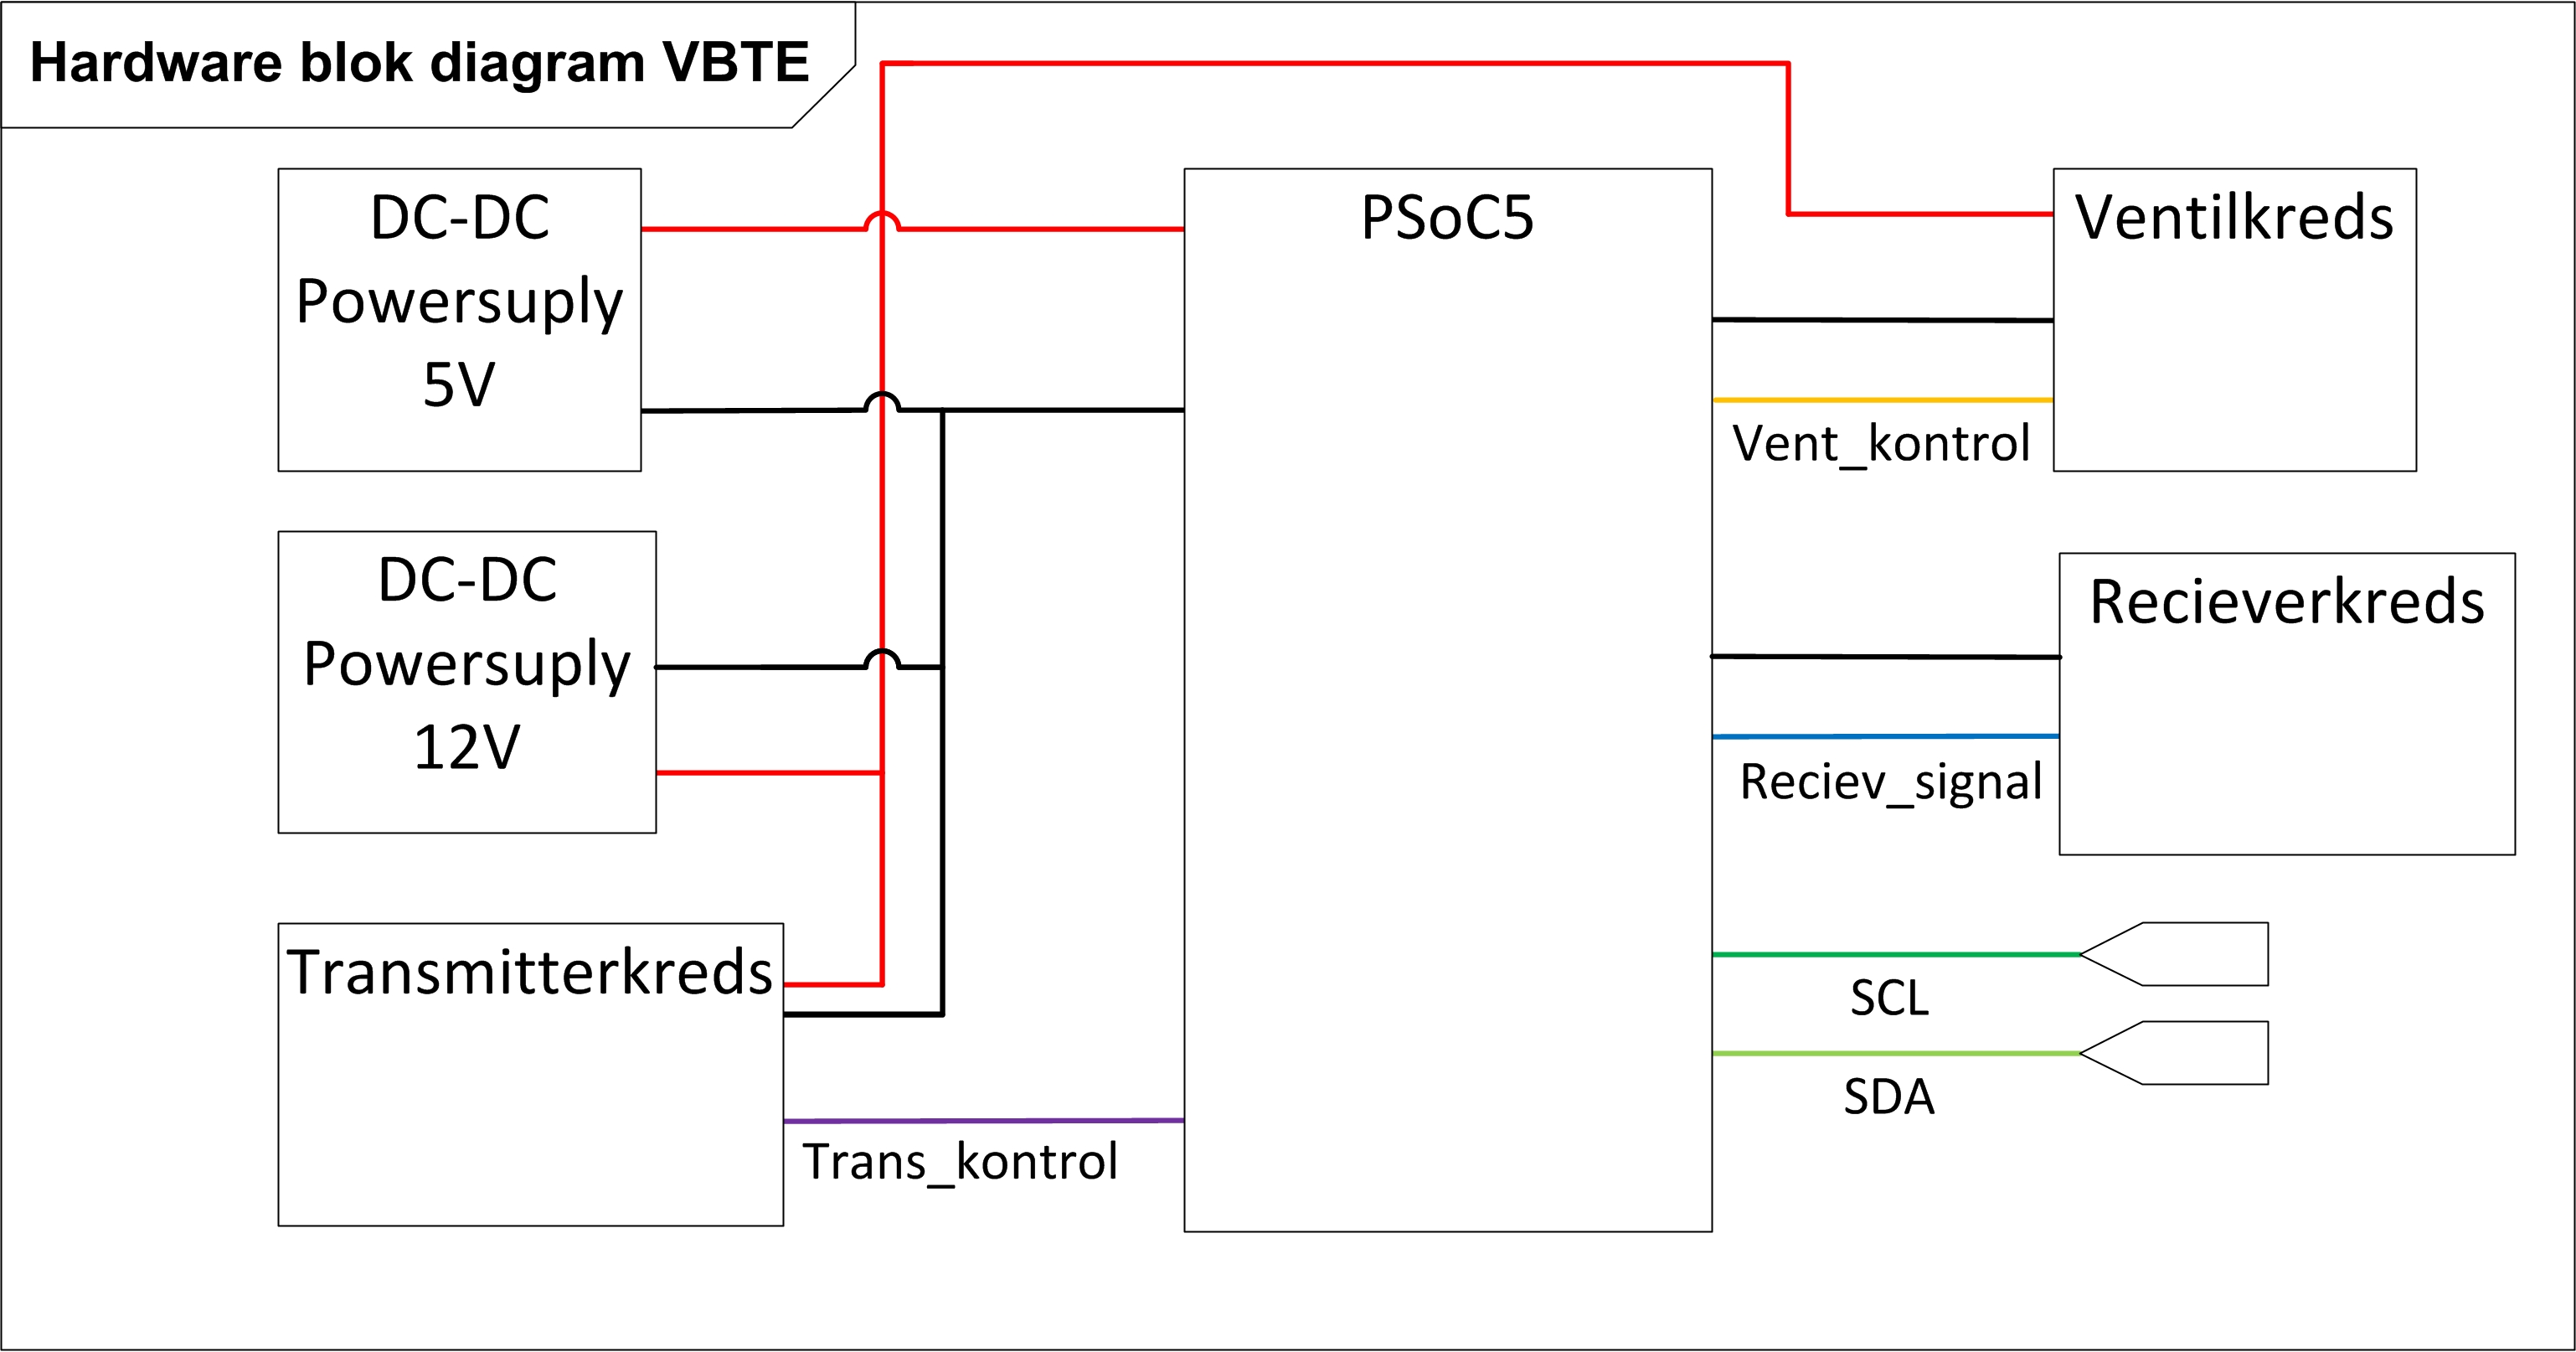
\includegraphics[width=1\textwidth]{billeder/HWVBTE}
\caption{Overordnet blokdiagram for VBTE hardware}
\label{fig:HWVBTE}
\end{figure}
\subsection{Blokke}
Nedenfor beskrives de enkelte blokke illustreret på \textit{Figur~\ref{fig:HWVBTE}}
\subsubsection{PSoC5}
PSoC'en er den centrale del af VBTE'en og står for styringen af hele VBTE'en. Den består af:
\begin{itemize}
\item Microcontroller
\item PGA
\item Mixer
\item Timer
\item Clocks
\item I2C
\item Delta-Sigma ADC
\item Kontrolregister
\end{itemize}
PSoC'en er et færdigkøbt produkt og for detaljer om de enkelte blokke heri henvises der til databladet for PSoC5.
\subsubsection{DC-DC powersuply 5V}
Se powersuply afsnittet.
\subsubsection{DC-DC powersuply 12V}
Se powersuply afsnittet.
\subsubsection{Transmitterkreds}
Transmitterkredsen består af en BD139 transistor samt en keramisk ultralydstransmitter af model 400ST. Kredsen bliver drevet af 12V powersuply.
\subsubsection{Reciverkreds}
Recierkredsen består af en keramisk ultralyds reciver(Model: 400SR).
\subsubsection{Ventilkreds}
Ventilkredsen består af en to transistorer, BD139 og BC547B, i en darlington kobling samt to ventier af model EV210A-1.2 og EV210A-4.5.
\newpage
\section{Nedbrydning af blokke}
Nedenfor følger nedbrydningen af de enkelte blokke med henblik på at designe de enkelte dele til systemet. Nedbrydningen sker for at gøre designet nemmere og mere overskueligt.
\subsection{PSoC5}
På \textit{Figur \ref{fig:PSoCBlok}} ses HW-designet internt på PSoC'en. De enkelte blokke bliver beskrevet efterfølgende.
\begin{figure}[H]
\centering
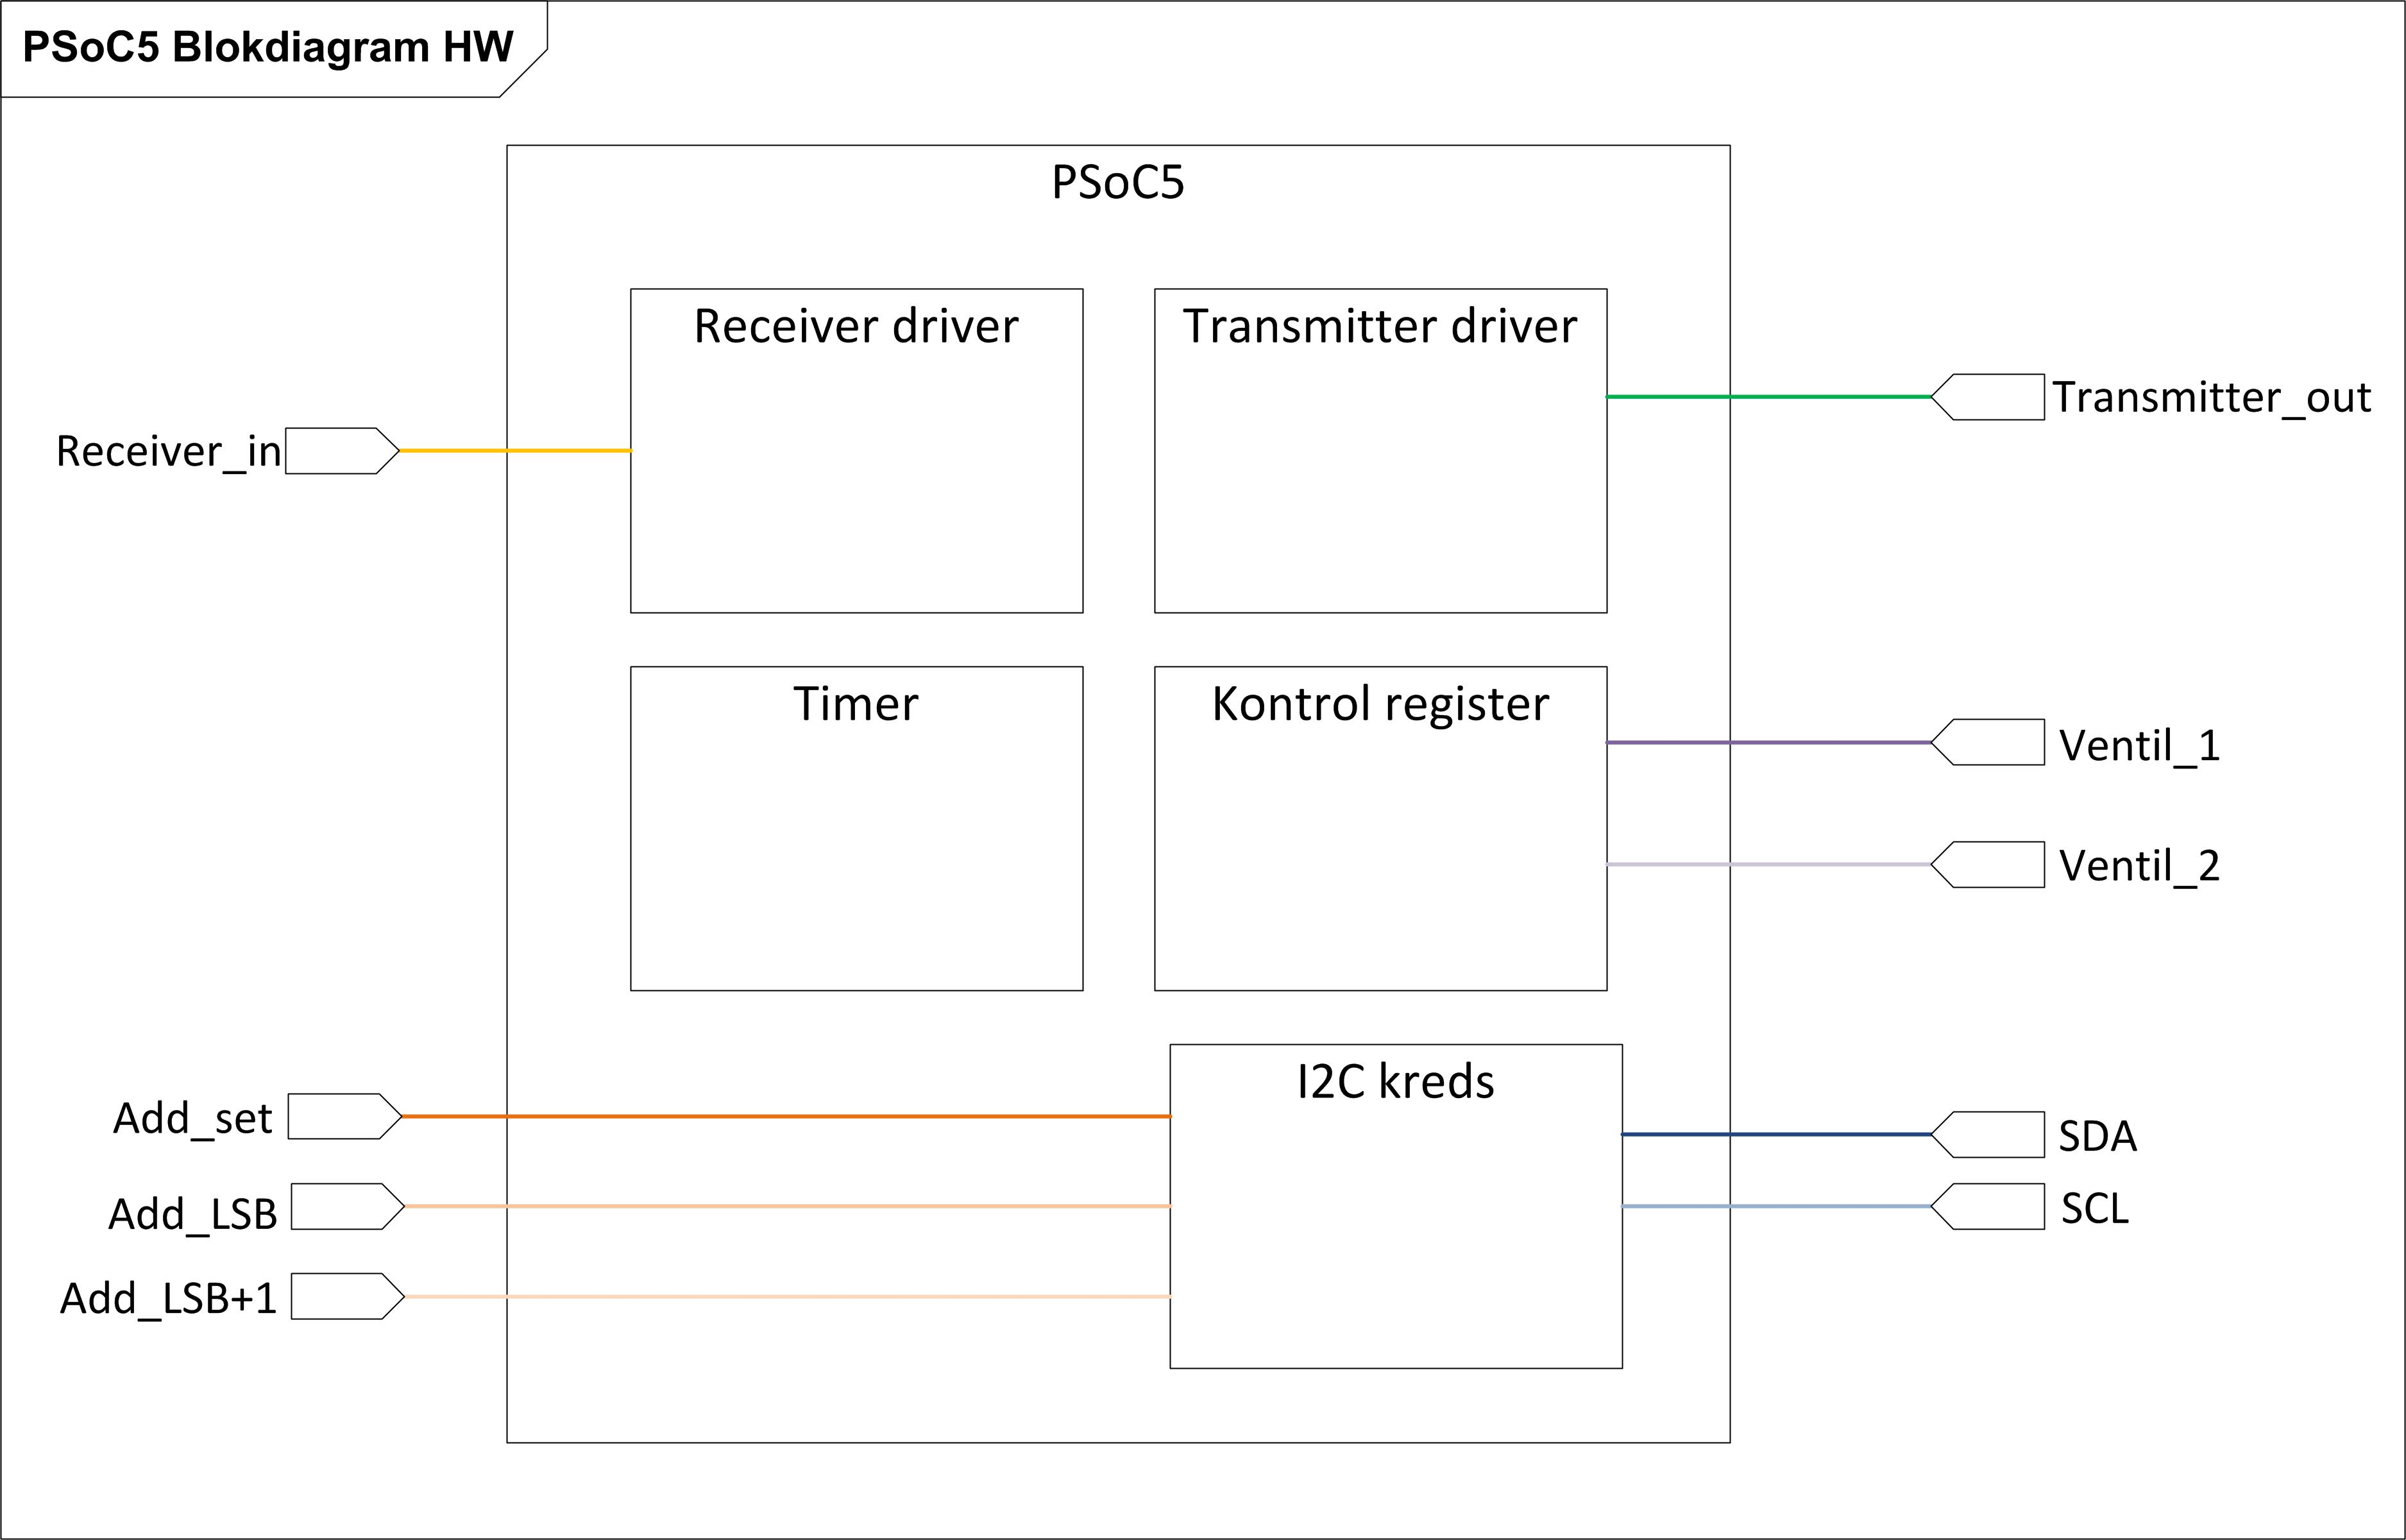
\includegraphics[width=1\textwidth]{billeder/PSoCBlock}
\caption{PSoC5 blokdiagram}
\label{fig:PSoCBlok}
\end{figure}
\subsubsection{Signalbeskrivelser:}
For signalbeskrivelser se \textit{tabel \ref{table:PSoCSignaler}}.
\fxnote{OPDATER TABELLEN!!!!}
\begin{table}[H]
\begin{tabular}{|p{3cm}|p{3cm}|p{3cm}|p{4.5cm}|} \hline
\cellcolor[gray]{0.85}Signal navn& \cellcolor[gray]{0.85}Type &\cellcolor[gray]{0.85}Spænding&\cellcolor[gray]{0.85}Beskrivelse\\ \hline
Receiver\_in & Analog (AC = 40kHz) & Ligger fra ca 0.01V til 0.3V & Spænding genereret i ultralydsreceiveren.\\ \hline
Trans\_kontrol & Analogt (AC = 40kHz) & ~0V til ~5V & Signal der skal styre ultralydstransmitteren \\ \hline
Ventil\_ind & Digitalt & ~0V til ~5V & Signal der skal styre ventilen til at lukke vand ind med.\\ \hline
Ventil\_ud & Digitalt & ~0V til ~5V & Signal der skal styre ventilen til at lukke vand ud med.\\ \hline
SDA & Digitalt & ~0V til ~5V & Et digitalt signal mellem VBTE og SM hvor I2C data læses fra.\\ \hline
SCL & Digitalt & ~0V til ~5V & Digitalt clocksignal til I2C.\\ \hline
\end{tabular}
\caption{Tabel over signaler i PSoC blokken}
\label{table:PSoCSignaler}
\end{table}
\subsubsection{Blokbeskrivelser:}
\subsubsection{Timer}
Timeren skal holde øje med tiden. Dette skal ske ved at timeren skal køre hele tiden. Der bliver læst timerværdien når et burst bliver sendt og når et burst bliver modtaget. Timeren skal derfor have en forholdsvis hurtig clock for at kunne gøre afstandsmålingen hurtig nok.
\subsubsection{I2Cdriver}
I2C kredsen skal stå for I2C interfacet mellem SM og VBTE. I2C protokollen kører 5V og med pull-up modstande. Denne del håndteres dog på SM da der kun er en instans af denne. I2C'en benytter standard I2C protokol og for yderligere info om data henvises der til \textit{Systemarkitektur/protokoller/I2C}.
\subsubsection{Receiverdriver}
Receiver driveren modtager signalet fra ultralydsrecieveren. Signalet skal, når det modtages, løftes op til 2.5V for at det kan anvendes på PSoC'en samt forstærkes. Det er vigtigt at signalet bliver tydeligt nok til at man kan være sikker på at man har modtaget en detektion. 
\subsubsection{Transmitterdriver}
Det er vigtigt for transmitteren at frekvensen ligger ret præcist da den dæmper signalet rigtigt meget ved frekvenser der ikke ligger ret langt væk fra 40kHz. For at timingen skal virke skal der også laves så der kan stoppes når der er sendt 10 perioder.
\subsubsection{Ventildriver}
Ventil driveren er den mest simple driver. Denne skal blot bære et digitalt signal til ON og OFF på hhv. ventilen til at lukke vand ind og ventilen til at lukke vand ud.

\subsection{Transmitterkreds}
På \textit{figuren \ref{fig:transmitterblok}} ses nedbrydningen af Transmitter kreds-blokken. Transmitterkredsen omsætter et kontrolsignal fra PSoC'en til et ultralyds signal.
\begin{figure}[H]
\centering
\includegraphics[scale=1]{billeder/transmitterblok}
\caption{På figuren ses transmitter blokken nedbrudt}
\label{fig:transmitterblok}
\end{figure}
\subsubsection{Signalbeskrivelser}
Signalerne internt i transmitter kredsen ses i \textit{tabel \ref{table:transmitterblok}}
\begin{table}[H]
\begin{tabular}{|p{3cm}|p{3cm}|p{3cm}|p{4.5cm}|} \hline
\cellcolor[gray]{0.85}Signal navn& \cellcolor[gray]{0.85}Type &\cellcolor[gray]{0.85}Spænding&\cellcolor[gray]{0.85}Beskrivelse\\ \hline
Trans\_kontrol & Digitalt & 0V - 5V & Modtages fra PSoC'en og skal omsættes til en større spænding over ultralydstransmitteren.\\ \hline
Trans\_out & Analogt (lyd) & 120dB \footnote{Aflæst fra datablad 400SRT 160} & Dette signal er lyden fra ultralydstransmitteren der sendes mod vandet og reflekteres tilbage til receiveren. \\ \hline
12V forsyning & Analogt DC & 12V$\pm$0.1V & 12V forsyning der leveres for powersupplyen beskrevet under powersupply.\\ \hline
GND & Ground & 0V & Ground i systemet \\ \hline
\end{tabular}
\caption{Tabel over signaler i Transmitterblokken}
\label{table:transmitterblok}
\end{table}

\subsection{Ventilkreds}
\label{sec:ventilkreds}
Ventil kredsen får to kontrolsignaler fra PSoC'en der skal åbne for hver sin ventil. Kredsen skal sørge for at ventilerne kan få lov til at trække den strøm der er nødvendig for at drive dem. På \textit{figur \ref{fig:ventilblok}} ses blokdiagrammet for ventilkredsen. Signalerne på blokdiagrammet er beskrevet i \textit{tabel \ref{table:ventrilkreds}}
\begin{figure}[H]
\centering
\includegraphics[scale=1]{billeder/ventilblok}
\caption{På figuren ses ventilblokken nedbrudt}
\label{fig:ventilblok}
\end{figure}
\begin{table}[H]
\begin{tabular}{|p{3cm}|p{3cm}|p{3cm}|p{4.5cm}|} \hline
\cellcolor[gray]{0.85}Signal navn& \cellcolor[gray]{0.85}Type &\cellcolor[gray]{0.85}Spænding&\cellcolor[gray]{0.85}Beskrivelse\\ \hline
Ventil\_1\_kontrol & Digitalt & 0V - 5V & Modtages fra PSoC'en og skal omsættes til en større spænding over ventilen.\\ \hline
Ventil\_2\_kontrol & Digitalt & 0V - 5V & Modtages fra PSoC'en og skal omsættes til en større spænding over ventilen.\\ \hline
Ventil\_1\_out & Digitalt & 0V - 12V & Udgangsspænding til ventilen.\\ \hline
Ventil\_2\_out & Digitalt & 0V - 12V & Udgangsspænding til ventilen.\\ \hline
12V forsyning & Analogt DC & 12V$\pm$0.1V & 12V forsyning der leveres for powersupplyen beskrevet under powersupply.\\ \hline
GND & Ground & 0V & Ground i systemet \\ \hline
\end{tabular}
\caption{Tabel over signaler i Transmitterblokken}
\label{table:ventrilkreds}
\end{table}
\newpage
\section{Opbygning af design}
Nedenfor følger opbygningen af designet for de forskellige kredse. Dette vil blive beskrevet med Multisim designs, PSoC designs og udregninger. Afsnittet vil starte med at beskrive PSoC designet, da dette er den mest centrale del af VBTE modulet.

\subsection{PSoC5 design opbygning}
I afsnittet om PSoC'en vil følge 5 underpunkter der beskriver hver blok som illustreret på \textit{figur \ref{fig:PSoCBlok}}.
\subsubsection{Timer}
Timeren er en indbygget timerblok i PSoC miljøet. Der er påkoblet en bus clock med en frekvens på 24MHz. Dette giver en opløsning på $\frac{1}{24MHz}*344\frac{m}{s}=0.014mm$\footnote{Dette er omtrent ved stuetemperatur ($20^{o}$)}. Timeren er sat op med 32bit som giver en wraparround tid på 3min for at der ikke skal bruges ekstra operationer i timingen på at tjekke efter wraparround. Nedenfor ses timerkredsen.
\begin{figure}[H]
\centering
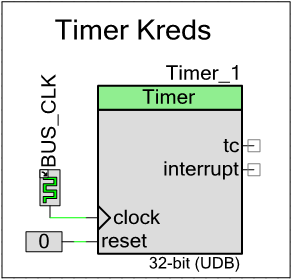
\includegraphics[scale=.5]{billeder/psoctimerkreds}
\caption{PSoC timerkreds.}
\label{fig:timerkreds}
\end{figure}
\subsubsection{I2Ckreds}
I2Ckredsen er en indbygget I2Cblok i PSoC miljøet. Den er sat som slave så SM modulet kan skrive til den og læse fra den. datahastigheden er sat til at køre 100kbps. Blokken har 2 udgange som er direkte forbundet til ben på PSoC'en. Disse er videre forbundet til et minijack hunstik der så den nemt kan kobles sammen med resten af systemet. Derudover er adressen sat i softwaren. Det er dog muligt at sætte LSB og LSB+1 i adressem i testdesignet. I det endelige system er det tænkt at de skal være sat op med en bestemt adresse fra start. På \textit{figur \ref{fig:psoci2ckreds}} ses blokken.
\begin{figure}[H]
\centering
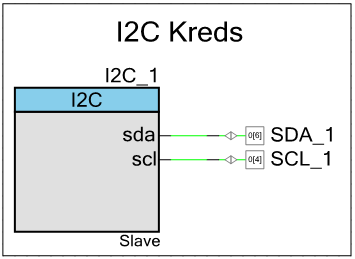
\includegraphics[scale=.5]{billeder/psoci2ckreds}
\caption{PSoC I2Ckreds.}
\label{fig:psoci2ckreds}
\end{figure}
\subsubsection{Receiver Driver}
Receiverdriveren består af en række indbyggede blokke i PSoC'en. Udover designet opbygget i PSoC miljøet er der en kondensator på 1µF, for at fjerne DC på ultralydsreceiveren, og en modstand der forbinder Opamp'en og PGA'en. Opamp'en er indsat for at løfte signalet op til 2,5V da PSoC'en ikke kan arbejde med negative spændinger. PGA'en forstærker herefter signalet op fra receiveren. Under teknologiundersøgelsen viste det sig at der blev modtaget en maks p-p værdi på 300mV på ultralydsreceiveren. Ud fra denne værdi blev en forstærkning beregnet for at være inden for PSoC'ens arbejdsområde\\
$A_{maks}*300mV+2.5V < 5V$. Anvendes en forstærkning på 8 fås et maks udsving på $300mV*8+2.5V=4.9V$.\\
Dette er dog kun hvis der modtages et meget klart signal og det er derfor en forstærkning på 8 godt kan anvendes. Signalet mixes  herefter sammen med et 40kHz signal\footnote{Den grønne streg er en forbindelse til den 40kHz clock der også anvendes i transmitterdriveren} for at få en DC ind på filteret i Delta-sigma AD konverteren. Den forventede spænding på ADC'en vil matematisk regnes til:\\
$U_{mixer}=\frac{1}{2}*A_{signal}*A_{clock}*A_{filter}=2.5V*\frac{1}{2}=1.25V$\footnote{Bemærk at dette er ved maksimalt udsving. Efterfølgende viste det sig at en lavere spænding også var detekteringer og grænset blev sat ved 0.3V}\\
Filteret i delta-sigma AD konverteren er designet i PSoC'en som et 3 ordens filter hvis første tap ligger ved samplingsfrekvensen. Samplingsfrekvensen er udregnet til at give filteret en opladningstid i 3dB punktet på $1/4ms$. Dette skyldes at de 10 perioder der bliver sendt varer $1/4ms$. Derved må der konstateres en detektion når filteret er opladet til 63\%. Delta-sigmaens dynamikområde er sat til $Vdda/2\pm1.25V$.\\
Udregning af samplefrekvens:\\
$\frac{1}{a}=\tau$, $\tau=250\mu s$ derved er $a=\frac{4000\frac{rad}{s}}{2*\pi}=637\si{Hz}$. \\
Dette giver en samplefrekvens på: $sps=3*637\si{Hz}=1910\si{Hz}$.\\
Nedenfor ses det endelige receiverdriver PSoC design. De forskellige parametre beregnet ovenfor er indsat i de forskellige blokke.
\begin{figure}[H]
\centering
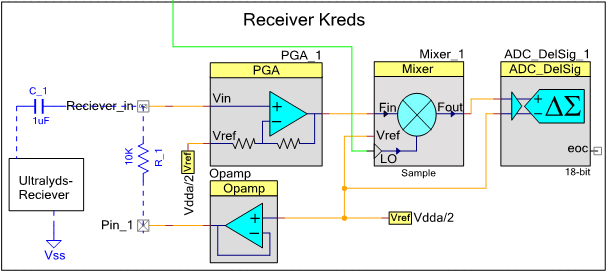
\includegraphics[scale=.75]{billeder/psocreceiverkreds}
\caption{PSoC receiverkreds }
\label{fig:psocreceiverkreds}
\end{figure}
\newpage
\subsubsection{Ventildriver}
Ventil driveren består af to software styrede output pins. Disse anvendes som kontrolsignal til Ventil Kredsen. Pinsne kan maks trække en strøm på 4mA. Nedenfor ses den endelige ventildriver på PSoC'en. 
\begin{figure}[H]
\centering
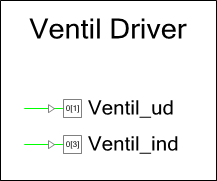
\includegraphics[scale=.5]{billeder/psocventildriver}
\caption{PSoC ventildriver}
\label{fig:psocventildriver}
\end{figure}

\subsubsection{Transmitterdriver}
Transmitterdriveren består af en output pin til kontrol af transmitterkredsen, en interruptrutine til at tælle antallet af perioder der bliver sendt, en interruptrutine til at hjælpe med et nonblocking delay, en 40kHz og en 1kHz clock samt en softwarestyret kontrol pin (Burst\_pin). Når kontrolpinden bliver sat bliver clocken and'et igennem ud til interruptrutinen samt kontrolpinden. \\
Nedenfor ses det endelige PSoC design for transmitterdriveren.
\begin{figure}[H]
\centering
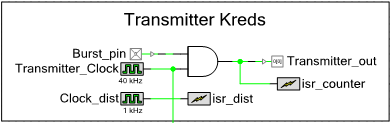
\includegraphics[scale=.8]{billeder/psoctransmitterdriver}
\caption{PSoC transmitterdriver}
\label{fig:psoctransmitterdriver}
\end{figure}
\newpage
\subsection{Transmitterkreds}
Transmitterkredsen skal, som beskrevet ovenfor, modtage et kontrol signal og omsætte det signal til en større spænding over den keramiske ultralydstransmitter. Dette er realiseret ved at anvende en transistor (BD139). I databladet aflæses impedansen af transmitteren til $\sim10k\Omega$ ved 40kHz. Med en forsyning på 12V trækker den derved en strøm på:\\
$I_{transmitter}=\frac{12V}{10k\Omega}=1.2mA$\\
Derved kan transistoren sagtens trække transmitteren og den er tilgængelig i lab.\\
På \textit{figur \ref{fig:transmitterkreds}} ses transmitterkredsen opbygget i multisim.

\begin{figure}[H]
\centering
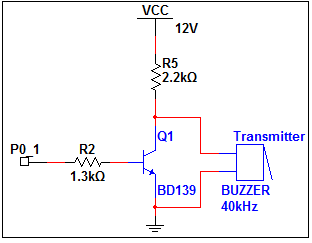
\includegraphics[scale=.75]{billeder/transmitterkreds}
\caption{Transmitterkreds i multisim}
\label{fig:transmitterkreds}
\end{figure}

\subsection{Ventilkreds}
Ventilkredsen skal, som beskrevet i punkt \ref{sec:ventilkreds} Ventilkreds, omsætte 2 kontrolsignaler til 2 outputs med en 12V spænding. Ventilerne er af typen EV210-1.2 og EV210A-4.5 fra danfoss og drives ved 12V 0.4A. Der er anvendt en darlington kobling af to transistorer for at trække en lille strøm fra PSoC'ens udgange. I koblingen er der anvendt en BC547B og en BD139. BD139 har en forstærkning på 40 - 160 (der regnes med 100) ifølge databladet. Derved skal der ligge en strøm på:\\
$I_{B}=\frac{0.4A}{100}=4mA$. \\
Ved en forsyning på 12V giver det en modstand på $R3=\frac{12V}{4mA}=3k\Omega$ men for at være sikre på at der bliver åbnet nok vælges en modstand på $1.2k\Omega$.
Dernæst skal der ligge en strøm på basen af den første transmitter på (forstærkningen i BC547B er på 200):\\
$I_{B2}=\frac{10m A}{200}=50\mu A$\\
Dette giver en modstand fra PSoC'en til basen på:\\
$R1=\frac{5V-1.4V}{50\mu A}=72k\Omega$\\
Denne afrundes til $70k\Omega$. På \textit{figur \ref{fig:ventilkreds}} ses opbygningen af designet i multisim.
\begin{figure}[H]
\centering
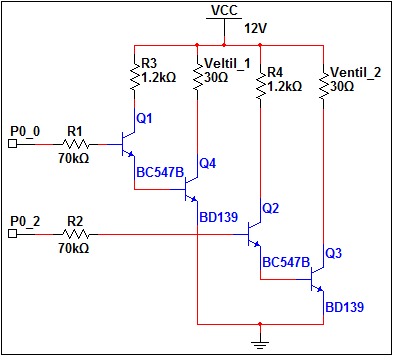
\includegraphics[scale=.75]{billeder/ventilkreds}
\caption{Ventilkreds i multisim}
\label{fig:ventilkreds}
\end{figure}
\section{Pin forbindelser}
Nedenfor ses pin forbindelser på PSoCen til VBTE designet.
\begin{table}[H]
\begin{tabular}{|p{3cm}|p{2cm}|p{8.5cm}|} \hline
\cellcolor[gray]{0.85}Signal navn& \cellcolor[gray]{0.85}Pin &\cellcolor[gray]{0.85}\cellcolor[gray]{0.85}Beskrivelse\\ \hline
SCL & P0\_4 & Clock til I2C \\ \hline
SDA & P0\_6 & Data til I2C \\ \hline
Trans\_kontrol & P0\_0 & Kontrolsignal til transmitter\\ \hline
Receiv\_in & P0\_2 & Receiver inputsignal\\ \hline
Ventil\_ind & P0\_3 & Kontrolsignal til ventilen der leder vand ind\\ \hline
Ventil\_ud & P0\_1 & Kontrolsignal til ventilen der leder vand ud\\ \hline

\end{tabular}
\caption{Tabel over pin forbindelser fra PSoC'en.}
\label{table:VBTEpinforbindelser}
\end{table}